\subsection{Strategy Description}
Basing on the analysis and results of section 4 and 5, we are profoundly aware of the central role that Sources play in the whole Drug Spread Model. Under the premises that the government management resources are limited, we hope to find an optimal strategy to maximize the control of drug spread while minimize the government resources used. 

Therefore, the strategy we take should mainly focus on Sources. To be more specific, we plan to:
\begin{itemize}
	\item Reinforce the drug investigation efforts in Source counties, hoping to decrease the amount of drug storage $S(t)$.
	\item Reinforce the intensity of inspection and control of private vehicles passing thorough cross-county road, hoping to limit the amount of drug transported from Sources to Consumers $T^{OUT}(t)$.
\end{itemize}

We make some adjustments on the existing Discrete Drug Spread Model in order to simulate and quantify drug spread. Considering the relationship between $S$ and $S'$ we discussed in equation (4-7), we assume that 
\begin{equation}
S'(t) = \delta S(t)
\end{equation}
where
\begin{equation}
\delta \sim U(0, 0.1)
\end{equation}

Corresponding to the strategy we proposed earlier, we add a storage control coefficient $\alpha$ and a transport control coefficient $\beta$, such that
\begin{equation}
\alpha S_i(t) - S_i'(t) = \lambda S_i(t) + \beta T_i^{OUT}(t), \alpha\in (0,1), \beta \in (1, +\infty)
\end{equation}
Combining (23-25), we have
\begin{equation}
(\alpha - \lambda - \delta)S_i(t) = \beta T_i^{OUT}(t), \alpha\in (0,1), \beta \in (1, +\infty)
\end{equation}
We set $\alpha$ in a range of $(0,1)$ because we hope that the storage after control $\alpha S(t)$ is smaller than that of the original storage. Similarly, we set $\beta > 1$ in that an increase in $\beta$ causes a decrease in $T^{OUT}$ when drug storage is known.

To test the effectiveness of this strategy, we focus on how the the change in $\alpha$ and $\beta$ influence storage.

\subsection{Evaluating the Strategy}
\subsubsection{Simulating Drug Spread}

\begin{wrapfigure}[13]{r}{0.2\linewidth} % Inline image example
	\begin{center}
		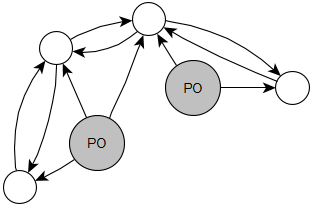
\includegraphics[width=\linewidth]{006}
	\end{center}
	\caption{Connection Between Possible Origins(PO) and Others}
\end{wrapfigure}

We simulate drug spread based on the directed graph we constructed in 4.2.1. We assume that drugs can be transported out of Origins, but not vice versa. Thus we delete all edges pointing towards Possible Origins in 4.2.1. 

We describe the simulation of drug spread as:

\begin{enumerate}[(1)]
	\item At $t=0$, we initialize the diagram by setting the storage of Origins to $S_i(0)=\gamma_i$, where $\gamma>0$ is a constant. We construct set VISITED = {} and push all Origins into VISITED. We initialize an all-zero array S\_RECORD, with a mapping from node index to array index.
	
	\item At $t=k, k>0$, S\_RECORD is again set to zero and the storage of Origins to $S_i(0)=\gamma_i$.(We assume that drug storage remains steady) For all nodes in set VISITED, we calculate their drug transportation to their out-neighbors using equation (9).For each node $i$, we add each $v_ij(t)$ to S\_Record[j]. After all nodes in the VISITED set were calculated, we add S\_Record[i] to $S_i$. After this, we traverse through the graph to add all nodes with $S>0$ but not yet in set VISITED into the set. 

\end{enumerate}

We compose a schematic diagram of storage flow. Inevitably, we will reach a point when all nodes are in the VISITED set. Simulation can carry on even when all nodes are visited. We visualize the spread in Figure 5:

\begin{figure}[H]
	\centering
	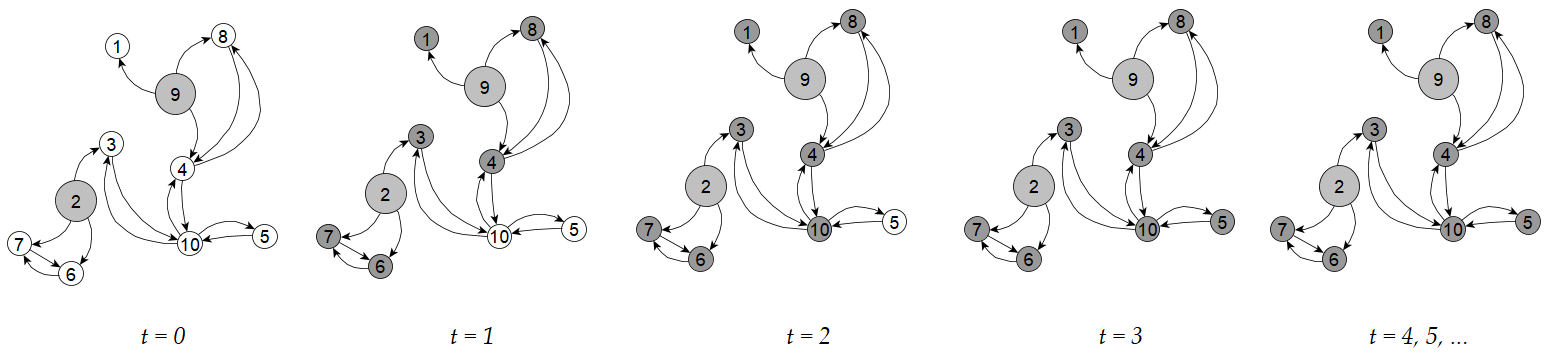
\includegraphics[width=\linewidth]{007}
	\caption{An Example Illustrating Drug Spread Simulation. \textit{Node 2 and 9 are Origins. White nodes indiates nodes never visited. Gray nodes are nodes in VISITED set.}}
\end{figure}

We assume that in year 2017, we have reached a point where all nodes are visited. Therefore, we have only to consider the change in $S_i$ for each node $i$ with the increment of $t$. 

\subsubsection{Evaluation Methods}
We evaluate our strategy both qualitatively and quantatively. 
\begin{itemize}
	\item Quantitative Method: using the threshold we proposed in Table Four, we hope that by controlling $\alpha$ and $\beta$, we could effectively reduce the number of first-level Sources and second-level Sources. Therefore, we define an ideal threshold $\mathcal{T}_1, \mathcal{T}_2$ to indicate an ideally low amount of first/second-level Sources, and compare how much time it takes for storage to change from the status in 2017 to our expected $\mathcal{T}_1, \mathcal{T}_2$ based on varying $\alpha$ and $\beta$. 
	
	\item Qualitative Method: we generate a heat map of drug storage at each time step $t$. Comparing these maps, we shall see the use-trend of opioids.
\end{itemize}

\subsubsection{Evaluation Results}

\subsection{Sensitivity Analysis: Identifing Significant Parameters}

--------------comment here -------------------------

To achieve a simulation as close to reality as possible, we suggest
\begin{itemize}
	\item In a short period of time, we assume that for Sources in each time period $[t,t+1)$, drug storage $S(t)$ remains a constaint. However,  
\end{itemize}

-------------ereh tnemmoc---------------------------